\section {Introduction}

L'objectif de cette cinquième tâche, conjointement avec la tâche quatre, était de nous sensibiliser aux risques dans l'industrie. Ce document traite de l'utilisation de soupapes de sécurité pour un tank d'ammoniac. Il offre des réponses aux questions qui nous ont été posées à ce propos. Nous parcourrons les conditions de stockage de l'ammoniac, dimensionnerons la surface de soupape et choisirons ainsi le type de soupape dont nous aurons besoin.

\section{Les soupapes de sécurité}
Une soupape de sécurité est un dispositif de sécurité très utilisé dans l'industrie. Les études \texsc{Hazop} indiquant qu'une surpression pourrait survenir dans une partie du système sont généralement à la base du placement de telles soupapes. Leur fonctionnement est le suivant: un ressort appuie sur un clapet, empêchant ainsi le fluide de sortir. Lorsque la pression devient trop importante, ce clapet s'ouvre et laisse passer le fluide, réduisant ainsi la pression. De telles soupapes doivent impérativement être correctement dimensionnées afin d'être optimales.

\section{Réponses aux questions concernant l'élément de sécurité}
\subsection{Pression normale de stockage (\unit{20}{\celsius})}

Comme observé sur la Figure \ref{graph1} la pression normale de stockage à \unit{20}{\celsius} est de \unit{8}{barg} (trait rouge).

\begin{figure}[ht!]
\centering
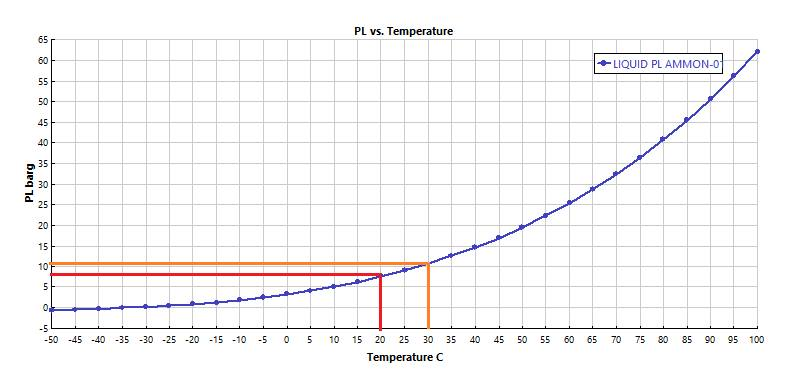
\includegraphics[scale=0.4]{tache5.jpg}
\caption{Pression $p_1$ vs. Température $T$}
\label{graph1}
\end{figure}

\subsection{Pression normale de stockage en été (\unit{30}{\celsius})}

De nouveau sur base de la Figure \ref{graph1} nous trouvons que la pression normale de stockage est de \unit{10}{barg} (trait orange).

\subsection{Pression maximale de tarage de la soupape}

Lors de sa conférence, monsieur \textsc{Minion} nous a expliqué que dans le cas d'un incendie, la pression maximale de tarage valait \numprint{121} \% de la pression de design. Rappelons que la pression de design est la pression pour laquelle l'équipement a été conçu. Dans notre cas, la pression de design du tank est de \unit{15}{b}; ce qui correspond à une pression de tarage de \unit{18}{barg}.

\subsection{Dimensionnement de la soupape}

Dans cette section nous allons dimensionner la soupape pour la pression de tarage décrite ci-dessus, c'est-à-dire \unit{18}{barg}.
Premièrement, nous avons déterminé que la pression durant la décharge, autrement dit la pression de tarage, était de \unit{18}{barg}. De nouveau grâce à la Figure \ref{graph1} nous avons pu trouver la température de sortie du liquide, à savoir \unit{45}{\celsius}.

Nous devons maintenant calculer la surface nécessaire pour l'orifice de la soupape et grâce à cela déterminer quelle soupape nous devrons commander, parmi celles disponibles sur le marché. Nous nous trouvons dans le cas d'une soupape sur un tank ne contenant qu'une seule phase gazeuse. A partir de ce constat nous pouvons utiliser la formule suivante qui nous permet de trouver la surface de la soupape:

\begin{equation}
A=\dfrac{W}{CK_dP_1K_bK_c}\cdot \sqrt{\dfrac{TZ}{M}}
\label{1}
\end{equation}

où $K_d=0.975$, $K_b=K_c=Z=1$\footnote{Données disponibles sur le site iCampus: \url{http://icampus.uclouvain.be/claroline/backends/download.php?url=L1RhY2hlXzVfZGltZW5zaW9ubmVtZW50X3NvdXBhcGUvTEZTQUIxNTAzX0RpbWVuc2lvbm5lbWVudF9QU1YucGRm&cidReset=true&cidReq=LFSAB1503}, "INTRODUCTION TO PRESSURE SAFETY VALVE (PSV) SIZING", consulté le lundi 8 décembre 2014}, $p_1$ vaut \numprint{121} \% de la pression de tarage (en \bbar), soit \unit{1925.175}{\kilo \pascal}, $T$ est la température pour une pression de \unit{18}{Barg} (voir Figure \ref{graph1}), $M$ la masse molaire de \ce{NH_3} soit \unit{17.031}{\gram \per \mole} et enfin $C$ et $W$ deux constantes à calculer. La première étape consiste donc à calculer $W$, le débit massique par heure de matière à évacuer. Par la relation suivante:

$$W=\dfrac{Q}{\Delta H_{vap}}$$

où $Q=C_1FA_{ws}^{0.82}$ avec $C_1=43200$, $F=1$, le facteur environnemental, et $A_ {ws}$ la surface mouillée \footnote{Calcul "élémentaire" sur base de la forme du tank} qui vaut \unit{48\pi}{\meter ^2} . En partant de là, nous trouvons que $Q=\unit{2779974753}{\joule \per \hour}$.

\begin{figure}[ht!]
\centering
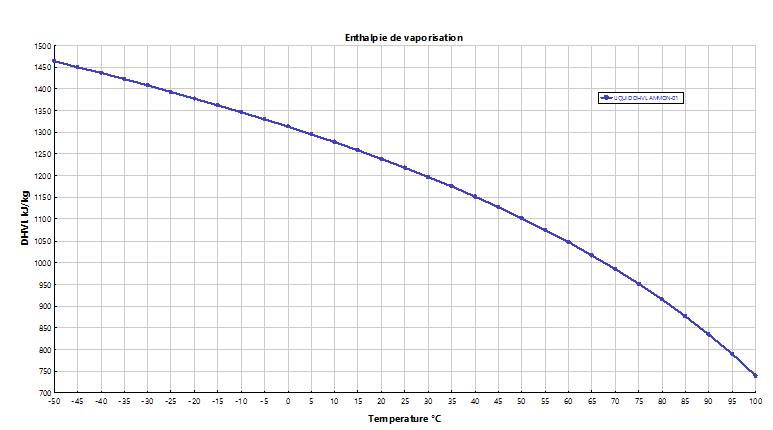
\includegraphics[scale=0.4]{tache51.jpg}
\caption{Enthalpie de vaporisation}
\label{graph2}
\end{figure}

Sur base de la Figure \ref{graph2} nous trouvons que $\Delta H_{vap}=\unit{1125}{\kilo \joule \per \kilo \gram}$ ce qui nous donne un débit de sortie de \unit{2471}{\kilo \gram \per \hour}.
Il nous reste donc à calculer la constante $C$:

$$C=0.03948\sqrt{k\left( \dfrac{2}{k+1}\right)^{\left( \dfrac{k+1}{k-1}\right)}}$$

où $K=\dfrac{C_p}{C_v}=1.33$, ce qui nous donne $C=0.02655$. En remplaçant le tout dans la formule \ref{1} on obtient une aire de \unit{2.10}{\centi \metre^2} soit \unit{0.32}{in^2}. Il reste maintenant à trouver dans le tableau (Figure \ref{tab}) à quelle soupape cela correspond. Nous en concluons qu'il nous faudra une soupape de type G.

\begin{figure}[ht!]
\centering
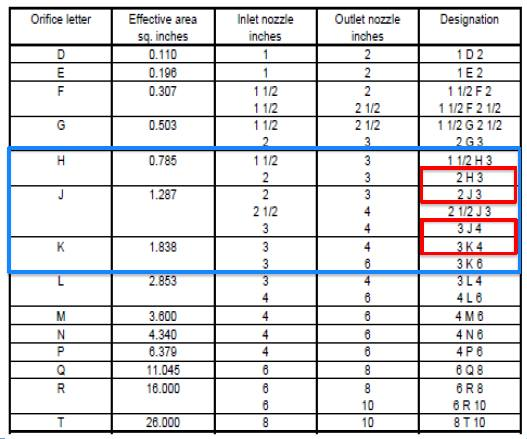
\includegraphics[scale=0.4]{tab.jpg}
\caption{Modèle standard de soupape}
\label{tab}
\end{figure}

\subsection{Tank avec une pression de design de \unit{20}{Barg}}
Si la pression de design de l’équipement était de 20 barg, le fait d’augmenter la pression de tarage de 5 bar et de la porter à 20 barg aura une influence sur le pression $p_1$, la température $T$ et sur la surface de la soupape.
Il suffit d'appliquer la même procédure que ci-dessus en changeant quelques données. En effet, la pression $p_1$ vaudra dans ce cas \unit{2553.39}{\kilo \pascal}, la température $T$ sera de \unit{50}{\celsius} (Voir Figure\ref{graph1}) et $\Delta H_{vap}=\unit{1100}{\kilo \joule \per \kilo \gram}$, cette valeur étant effectivement influencée par la température (Voir Figure \ref{graph2}). Le calcul de $A$ nous donnera une valeur de \unit{16.6}{\centi \metre^2}.

\subsection{Conséquence de l'isolation thermique du tank}

Nous revenons au cas du premier calcul de $A$, sauf que dans ce cas c'est le facteur environnemental $F$ qui sera différent et qui sera égal à \numprint{0.132}. Ce qui nous donne $A=\unit{0.28}{\centi \metre^2}$. Ce résultat est logique, car l'élévation de température à l'intérieur sera très faible voire inexistante pour un incendie.

\section{Conclusion}
Les questions qui nous ont été posées nous ont montré que la pression dans des tank d'ammoniac est variable, notamment en fonction des saisons et de la température. L'utilisation de soupapes de sécurité est quelque chose de très courant et c'est également une solution sûre étant donné que le processus se met en marche automatiquement. Le dimensionnement de ces soupapes est une démarche longue mais extrêmement importante parce qu'une soupape mal dimensionnée perd rapidement en efficacité. Dans le cas de notre production d'ammoniac, il nous faut des soupapes de type G pour une pression de \unit{18}{barg}.
